\documentclass[12pt]{article}
\usepackage[utf8]{inputenc}
\usepackage[T1]{fontenc}

\usepackage[english]{babel}
\usepackage{amsmath,amssymb,amsfonts}

\usepackage{xcolor}
\usepackage{graphicx}

\usepackage{caption}
\usepackage{subcaption}

%New colors defined below
\definecolor{codegreen}{rgb}{0,0.6,0}
\definecolor{codegray}{rgb}{0.5,0.5,0.5}
\definecolor{codepurple}{rgb}{0.58,0,0.82}
\definecolor{backcolour}{rgb}{0.95,0.95,0.92}

\usepackage{hyperref}
\hypersetup{
	colorlinks=true,
	citecolor=codegreen, 
	linkcolor=codegreen,
	filecolor=codepurple,      
	urlcolor=codepurple,
}

\usepackage{float}

%Margins
\usepackage{geometry}
\geometry{
	a4paper,
	total={190mm,277mm}, % a4 is 210 x 297 mm
	left=10mm,
	top=17mm,
}
\setlength{\parindent}{0pt}
\setlength{\parskip}{1pt}

%circuit tikz
\usepackage{circuitikz}

%%bibliography 
%\usepackage[backend=biblatex,style=science]{biblatex} %Imports biblatex package
%\addbibresource{spect.bib} %Import the bibliography file

%titlepage
\title{\color{blue}Q-meter experiment}
\author{Shashvat Jain}
\date{}
\begin{document}
	\begin{titlepage}
		\maketitle
		\begin{center}
			\vspace{10cm}
			Submitted to Dr. Daljeet Kaur\\
			"32223904 - BASIC INSTRUMENTATION SKILLS"
		\end{center}
		\tableofcontents
		\thispagestyle{empty}
	\end{titlepage}
	\newpage
	\section{Objective}
	Objective is to determine accurate \textbf{Quality Factor }of an unknown coil using the following arrangement.
	
	\section{Theory}
	The determination of the Quality factor $ Q $ using Q-meters is one of the most widely used means in the laboratory for testing radio frequency coils, inductors and capacitors.\\ The Quality factor is equal to $Q=\omega_0 L/R$ where $\omega_0$ is the resonant frequency, $ L $ is the inductance and $ R $ is the effective resistance of the a coil. 
	The effective resistance $ R $, is never determined directly since its value depends upon the value of frequency.
	\begin{figure}[H]
		\begin{circuitikz}[american, scale = 1.5][americanvoltages]
			\draw (0,0)
			to[V=$E$] (0,2) % The voltage source
			to[R, v^<=$R$] (2,2) % The resistor
			to[C, v^<=$C$] (2,0) % Capacitor 
			to[L, v^<=$L$] (0,0);% Inductor 
			
			%\draw[thin, <-, >=triangle 45] (1,1)node{$i_1$}  ++(-60:0.5) arc (-60:170:0.5);
		\end{circuitikz}
		\centering
	\end{figure}
	\section*{Principle of Working}
	
	The principle of working of this useful laboratory instrument is based upon the well-known characteristics of a resonant series R-L-C circuit.
	
	At resonant frequency $ f_0 $, we have $X_C = X_L$ where capacitive reactance $X_C = \frac{1}{2 \pi f_0 C}$, inductive reactance $X_L = 2 \pi f_0 L $ \\[2mm] and resonant frequency $f_0 = 1/(2 \pi \sqrt{LC})$ and current at resonance $I_0 = E/R$ is then given by
	
	The voltage across the capacitor $E_C=I_0 X_C=I_0X_L=I_0\omega_0L$ and input voltage $E=I_0*R$
then $E_C/E=(\omega_0 L)/R=Q$ and $E_C=QE$.
	
	If the input voltage is kept constant the voltage across capacitor is Q times E and a voltmeter connected across the capacitor can be calibrated to read the value of Q directly.

	\begin{figure}[H]
		\centering
		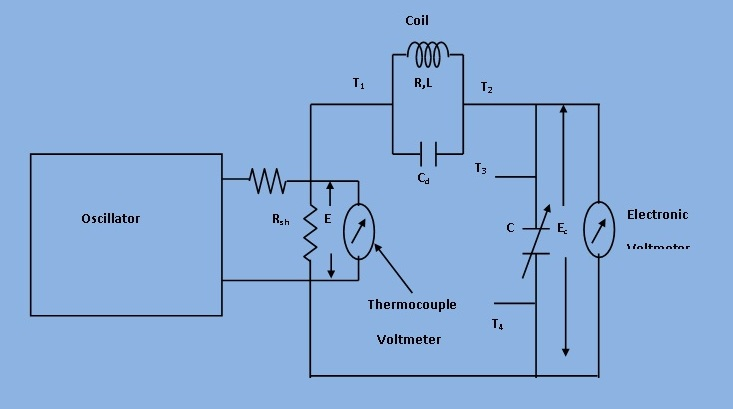
\includegraphics[scale= 0.7]{circuit.jpg}
		\caption{Circuit diagram for the arrangement of Q-meter}
	\end{figure} 

	\section{Procedure}
	\begin{enumerate}
		\item Set the Shunt Resistance (Rsh) value as small as possible (Say 0.02 Ohm). Set all the parameters (R, L, C) by yourself.
		\item Set the voltage value of the oscillator (E=10 V).
		\item At f=100 Hz. Check the value of voltage drop across capacitor. (EC).
		\item Change the frequency until EC reach at the maximum value. Then calculate the value Q measured using this formula $Q_{meas}=(\omega_0 L)/(R+ R_(sh))$.
		\item Calculate the true value of unknown coil by using this formula $Q_(true)=(\omega_0L)/R$
		\item First resonance occurs due to frequency (say f1). Note down the value of tuning capacitor C. (say C1). Double the input frequency (f1) (say f2=2*f1). Change the tuning capacitor value until resonance occurs. Note down the value of tuning capacitor C. (say C2). Discharge capacitance (Cd) would be =(C1-4*C2)/3. 
	\end{enumerate}
	\section{Result }
	We obtain the following readings for $ E=10V $,$ f_0 = 2700056 $ \\
	$ V_c=788.053581999041V $,$ Q_{true} = 8.9507164206384  $
\end{document}